%!TEX root = /home/glauffer/Dropbox/FURG/final_project/monografia/monografia.tex
\chapter{Resultados e Discussão}
\label{cap:resultados}
%Como mostrar os resultados de maneira eficiente

%\section{resultado parciais}
\section{Dados do Catálogo OGLE}

Em um total foram calculados os períodos de $25707$ estrelas variáveis localizadas na Grande Nuvem de Magalhães e pertencentes ao catálogo OGLE. Deste numero total, $3056$ eram Cefeidas clássicas tipo FO e FU, e $22651$ eram RRLyraes tipo AB e C. Os resultados obtidos foram comparados com os resultados do catálogo e o percentual de acertos, considerando uma precisão de $10^{-4}$, pode ser visto na tabela \ref{tab:resultados}.

\begin{table}
\begin{center}
\caption[Quantidade de dados analisados e resultados corretos.]{Quantidade de dados analisados e resultados corretos considerando uma precisão de $10^{-4}$.}
\begin{tabular}{c|c|c|c}
\toprule
Estrelas & Quantidade & Acertos  & Porcentagem \\
\midrule
Cefeidas FU & $1818$ & $1817$ & $99,94 \%$ \\
Cefeidas FO & $1238$ & $1231$ & $99,43 \%$ \\
%\hline
RRLyraes AB& $17693$ & $17540$ & $99,14 \%$ \\
RRLyraes C& $4958$ & $4535$ & $91,47 \%$ \\
\midrule
\textbf{Total} & $\textbf{25707}$ & $\textbf{25123}$ & $\textbf{97,73 \%}$ \\
\bottomrule
\end{tabular}
\label{tab:resultados}
\end{center}
\end{table}

De acordo com os resultados da tabela \ref{tab:resultados} podemos perceber que para as Cefeidas o método apresenta um resultado um pouco melhor se comparado com as RR Lyraes. Uma explicação para este resultado seria que o método de entropia de Shannon condicional funciona melhor para magnitudes mais brilhantes \citep{comparison}. Tendo em vista que as Cefeidas ($m \approx 15$) são mais brilhantes do que as RR Lyraes ($m \approx 19$), essa afirmação é coerente com os resultados. %e sendo as Cefeidas ($m \approx 15$) mais brilhantes do que as RR Lyraes ($m \approx 19$), essa afirmação é coerente com os resultados.  %ver faixa de magnitude da cefeidas e lyraes

A alta taxa de acerto do método nos informa que
com estes resultados podemos confiar no método de entropia de Shannon condicional, porém para entender melhor o comportamento desse método será analisado os resultados para dados sintéticos.

\section{Dados Sintéticos}

Dados sintéticos foram criados a fim de explorar o método e entender até onde podemos utilizá-lo, pois os sinais sintéticos são construídos com parametros que podemos controlar e modificar. De acordo com a tabela \ref{tab:resultados}, as RRLyraes apresentaram uma taxa menor de acerto, por essa razão elas foram utilizadas como referencia para construir os dados sintéticos. Para isto, é necessário entender os dados das RR Lyraes do catálogo OGLE para obter os parâmetro sobre o tempo e amostragem para enfim utilizar a expressão \ref{eq:dado_sint} e construir os dados.

Analisando os dados das $22651$ estrelas, foram criados histogramas sobre os dados iniciais e finais do tempo e a quantidade de pontos de observação. As figuras \ref{fig:hist} e \ref{fig:histo_n} nos mostram esses histogramas.

\begin{figure}[!h]
\centering
\begin{subfigure}{.5\textwidth}
  \centering
  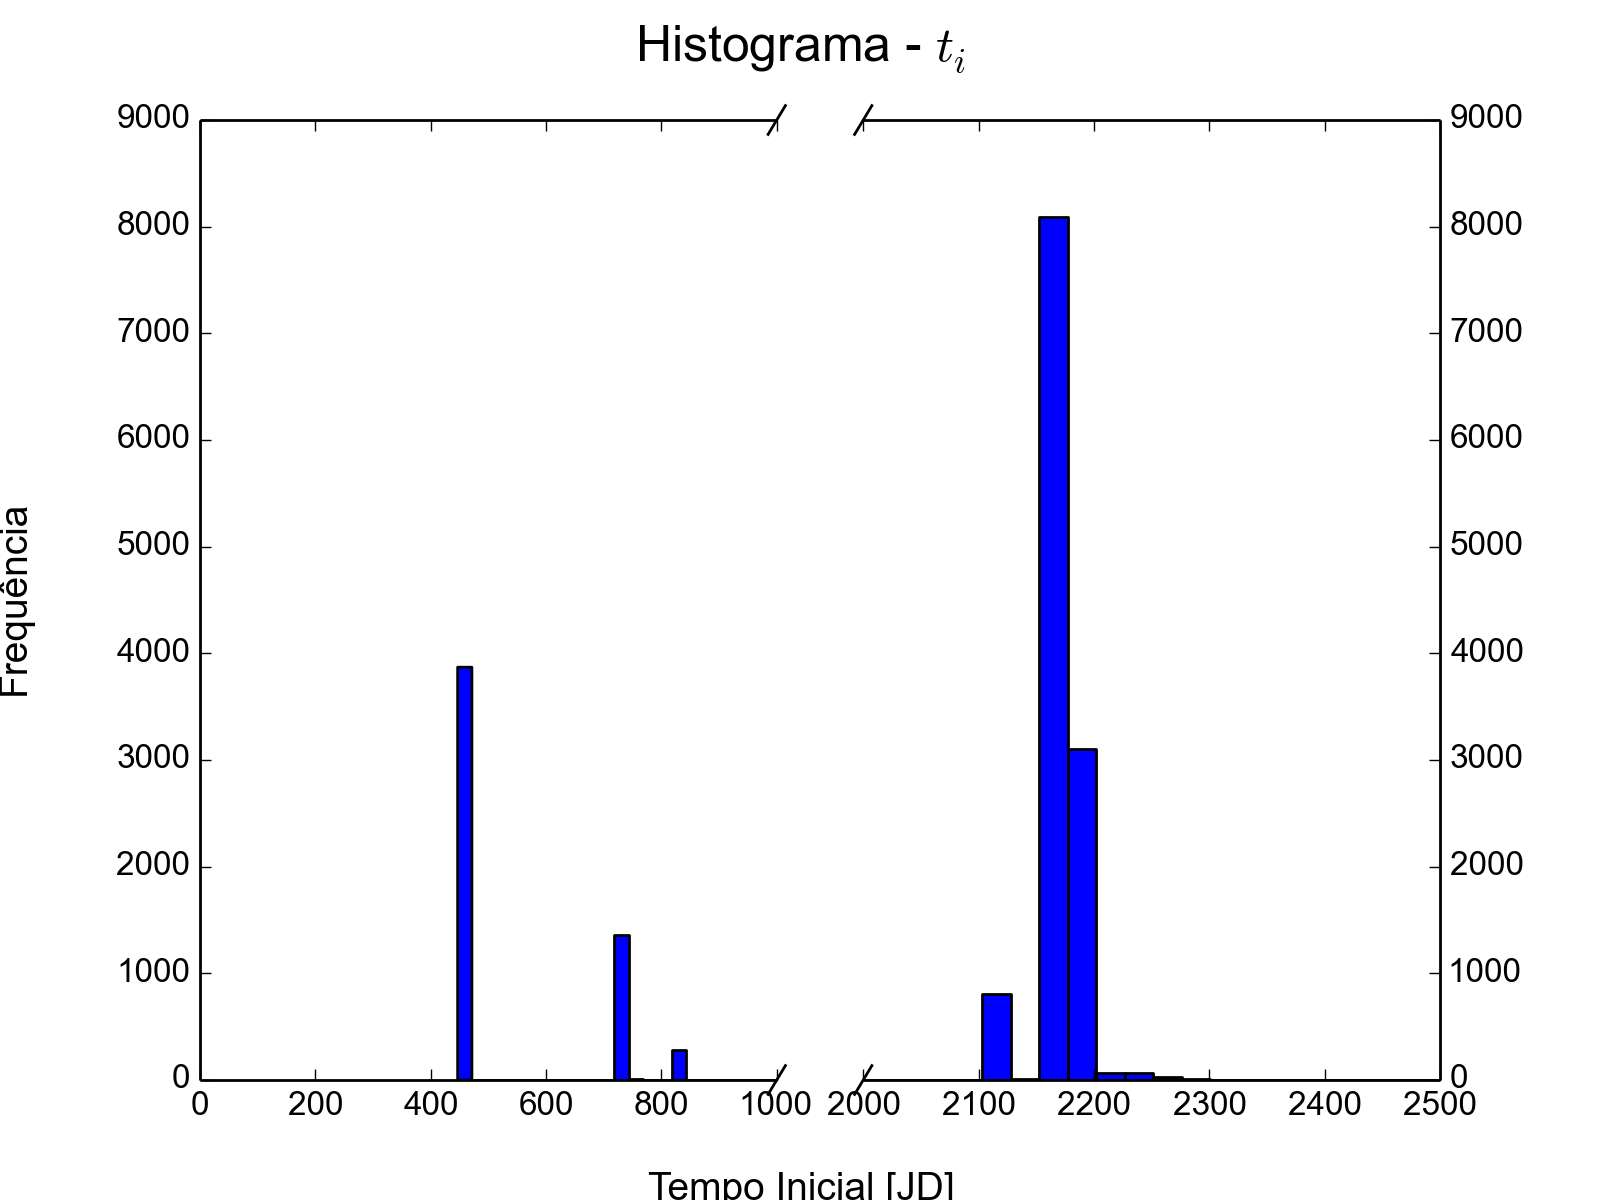
\includegraphics[width=\linewidth]{hist_ti.png}
  \caption{Tempo Inicial}
  %\label{fig:right}
\end{subfigure}%
\begin{subfigure}{.5\textwidth}
  \centering
  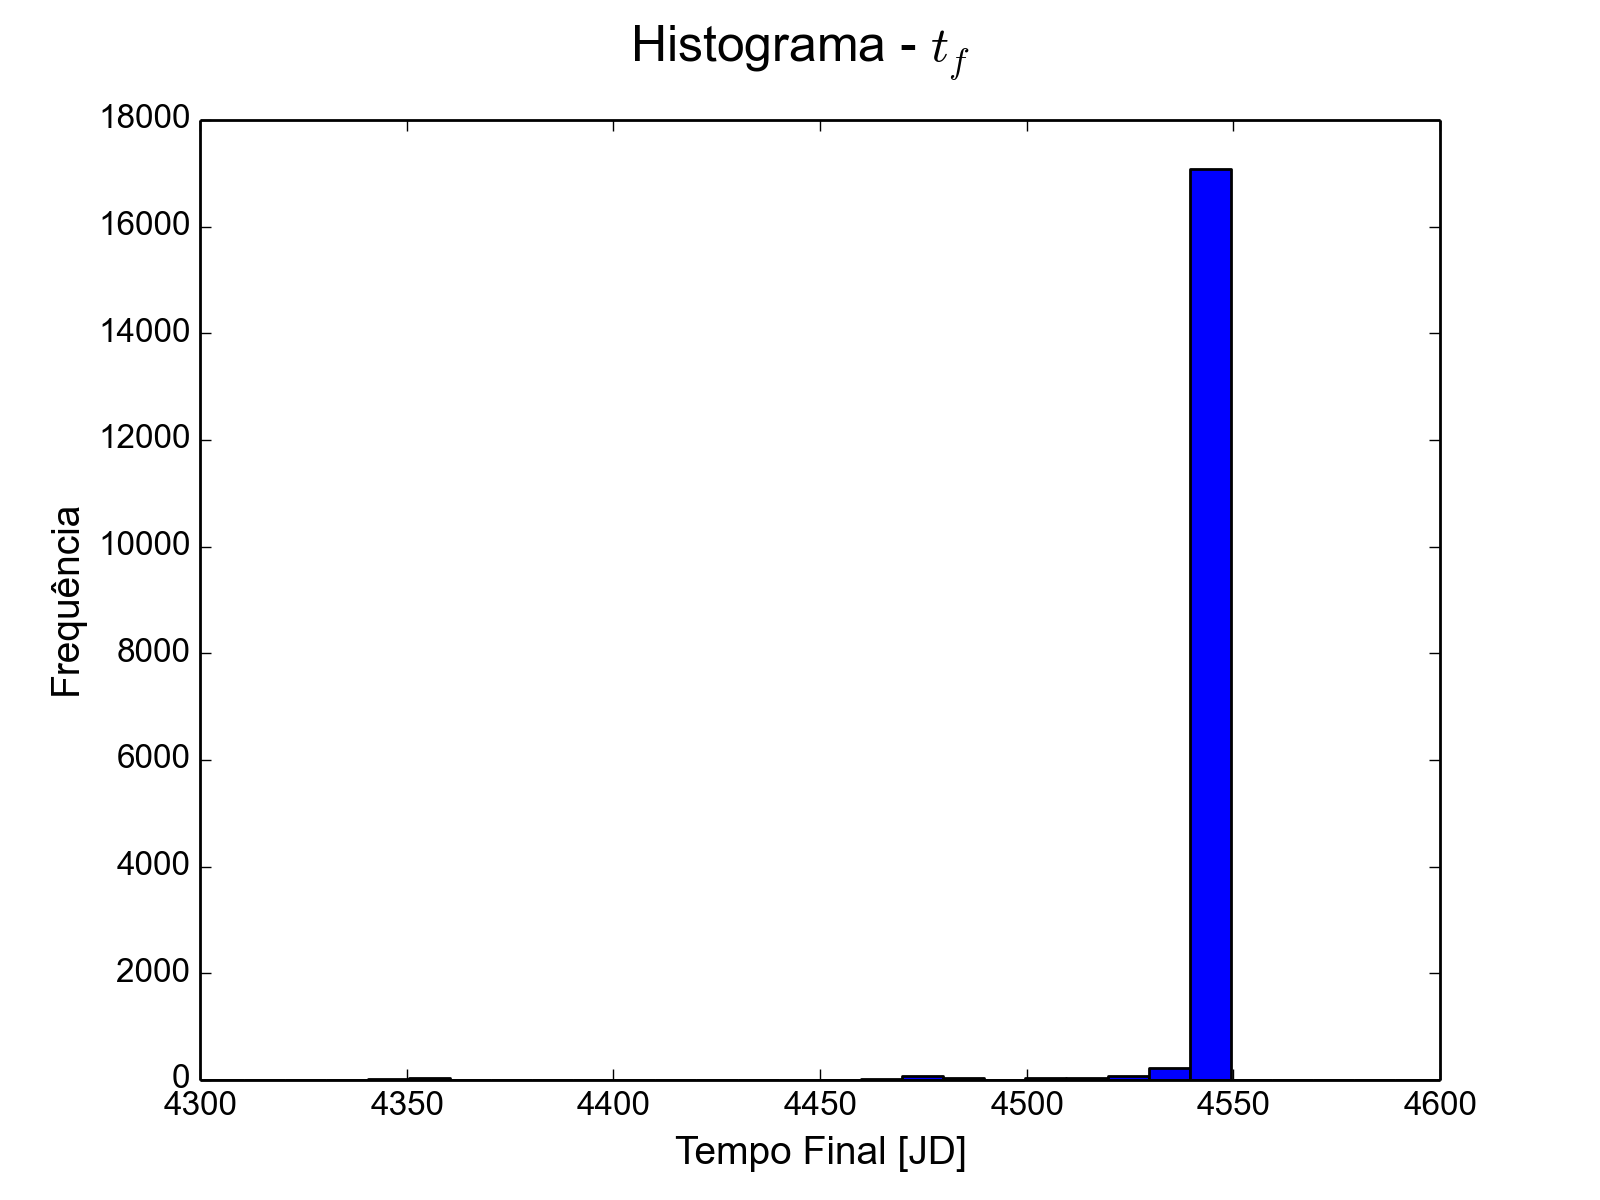
\includegraphics[width=\linewidth]{hist_tf.png}
  \caption{Tempo Final}
  %\label{fig:wrong}
\end{subfigure}
\caption[Histogramas sobre tempo inicial e final.]{Histogramas sobre o tempo inicial e final das RR Lyraes. As imagens representam (a) tempo inicial e (b) tempo final . A partir dessa análise foram obtidos os valores $t_i = 2152,5019$ e $t_f = 4539,4593$.}
\label{fig:hist}
\end{figure}

A partir dessa análise foram obtidos os valores $t_i = 2152,5019$ e $t_f = 4539,4593$ e $n = 352$ como os valores de tempo inicial, final e quantidade de pontos mais frequentes nos dados das RR Lyraes. Desta forma, utilizando esses valores é possível construir um sinal sintético que se assemelhe com os dados do catálogo. Então, a amostragem é calculada pela expressão \ref{eq:amostragem} em que a variação do tempo é obtida da seguinte forma:
\begin{align}
dt = \frac{t_f - t_i}{n} = \frac{4539,4593 - 2152,5019}{352} = 6,7888
\end{align}
E substituindo este resultado na equação \ref{eq:amostragem} teremos:
\begin{align}
f_s = 0,1473 .
\end{align}
Desta forma foi determinado, a partir dos dados do catálogo, qual a variação média entre os pontos de observação e foi calculada a amostragem média dos dados.

\begin{figure}[!ht]
  \centering
  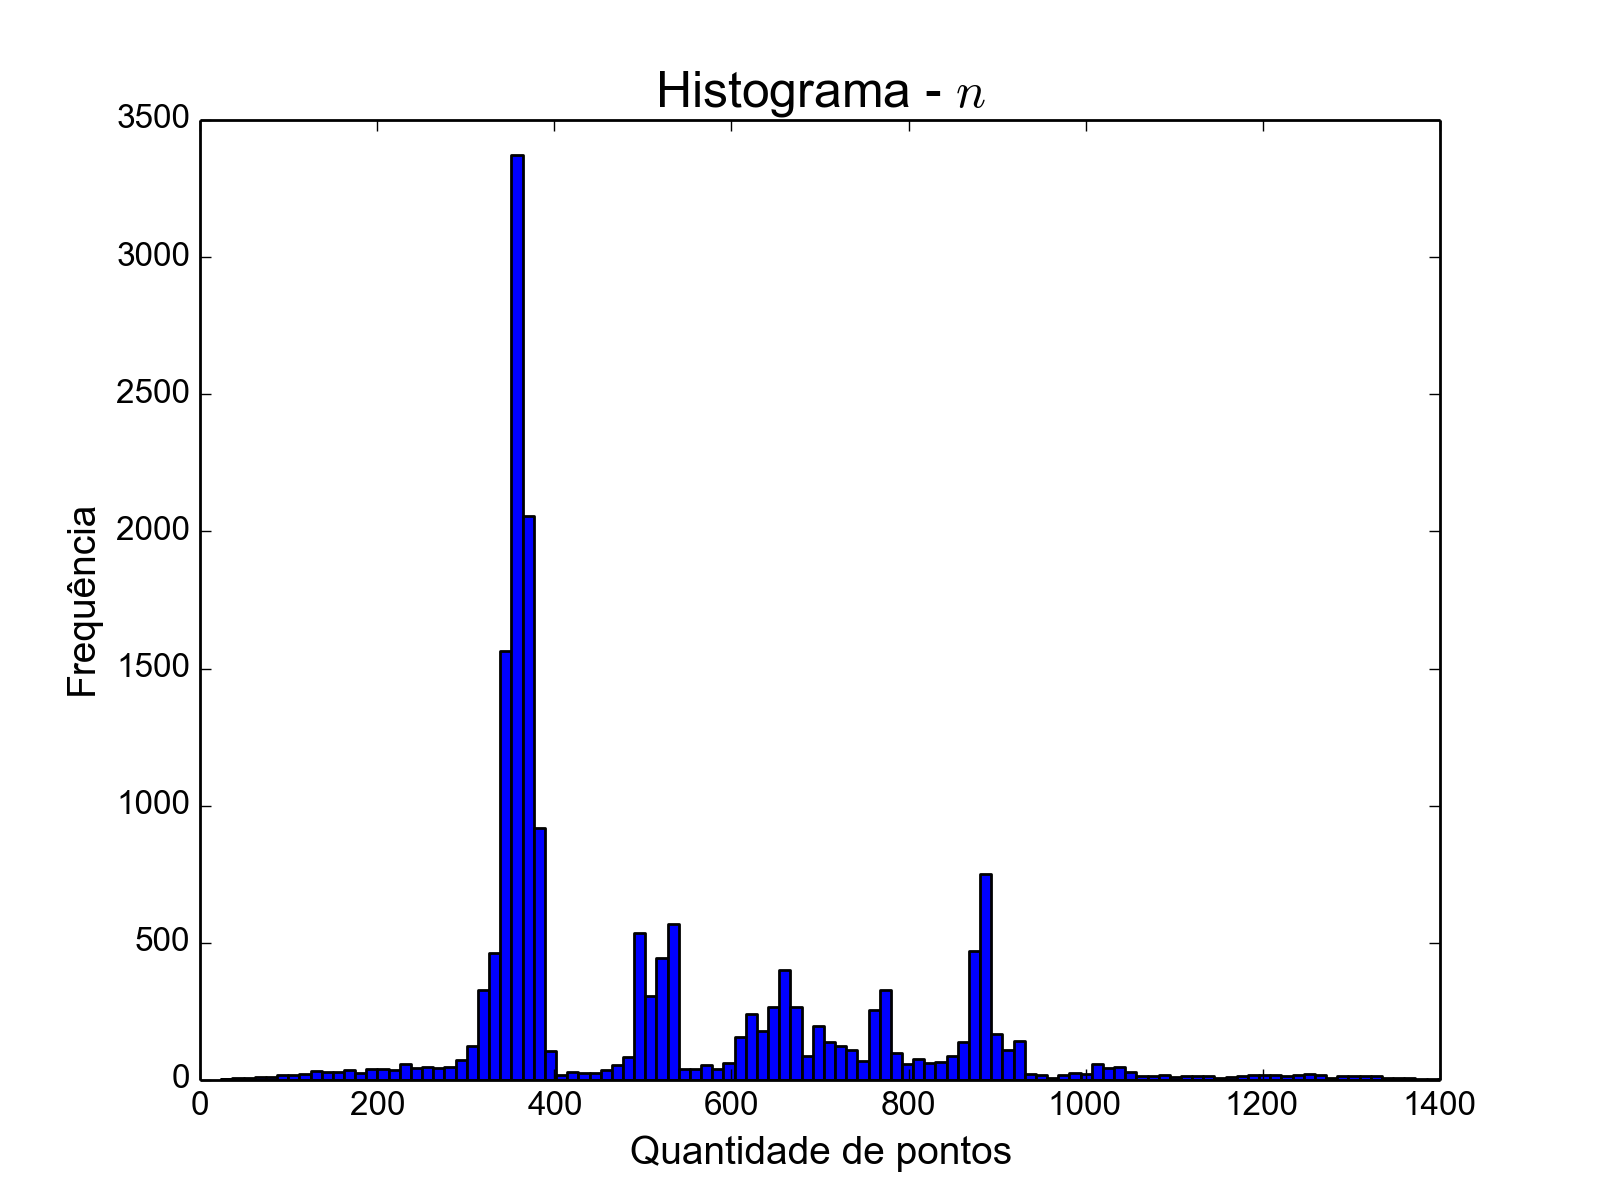
\includegraphics[width=0.6\linewidth]{hist_n.png}
  \caption[Histograma sobre quantidade de pontos.]{Histograma sobre a quantidade de pontos nos dados das RR Lyraes. A quantidade com maior frequência é $k = 352$.}
  \label{fig:histo_n}
\end{figure}

Tendo obtido a amostragem, podemos construir dados sintéticos variando a frequência de pontos e o nível de ruído para estudar como o método se comporta com esses sinais. O sinal sintético é construido pela expressão \ref{eq:dado_sint} em que os termos $A_i$ são dados por \citet{ce} e \citet{entropy} como sendo
$A_0 = 15$, $A_1 = -0.5$, $A_2 = 0.15$ e $A_3 = -0.05$ . O período utilizado para criar o sinal será $P = 0.576$ dias, pois de acordo com \citet{lyraes} esse é o valor de período médio das RR Lyraes do catálogo.

\begin{figure}[ht]
\centering
\begin{subfigure}{.5\textwidth}
  \centering
  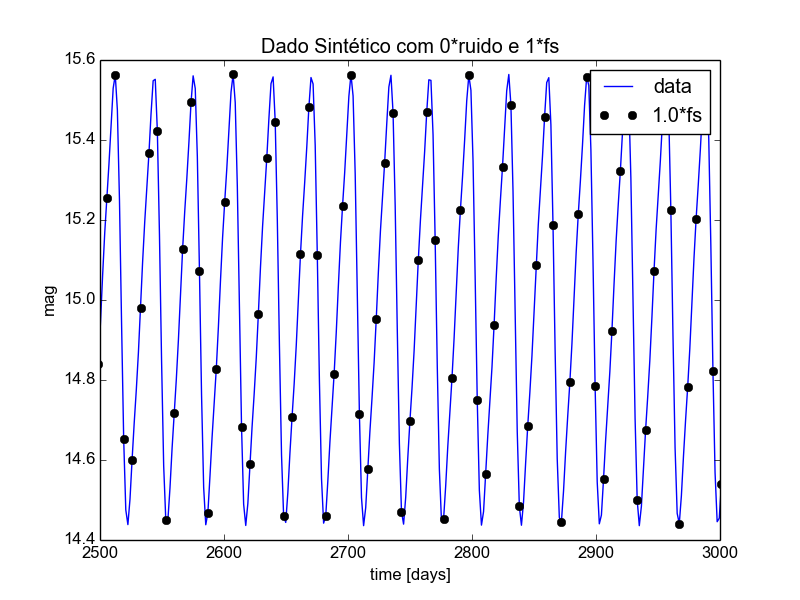
\includegraphics[width=\linewidth]{dado_sintetico_0_ruido_1_amos.png}
  \caption{Dado sem ruído e com amostragem padrão}
  \label{fig:1amos}
\end{subfigure}%
\begin{subfigure}{.5\textwidth}
  \centering
  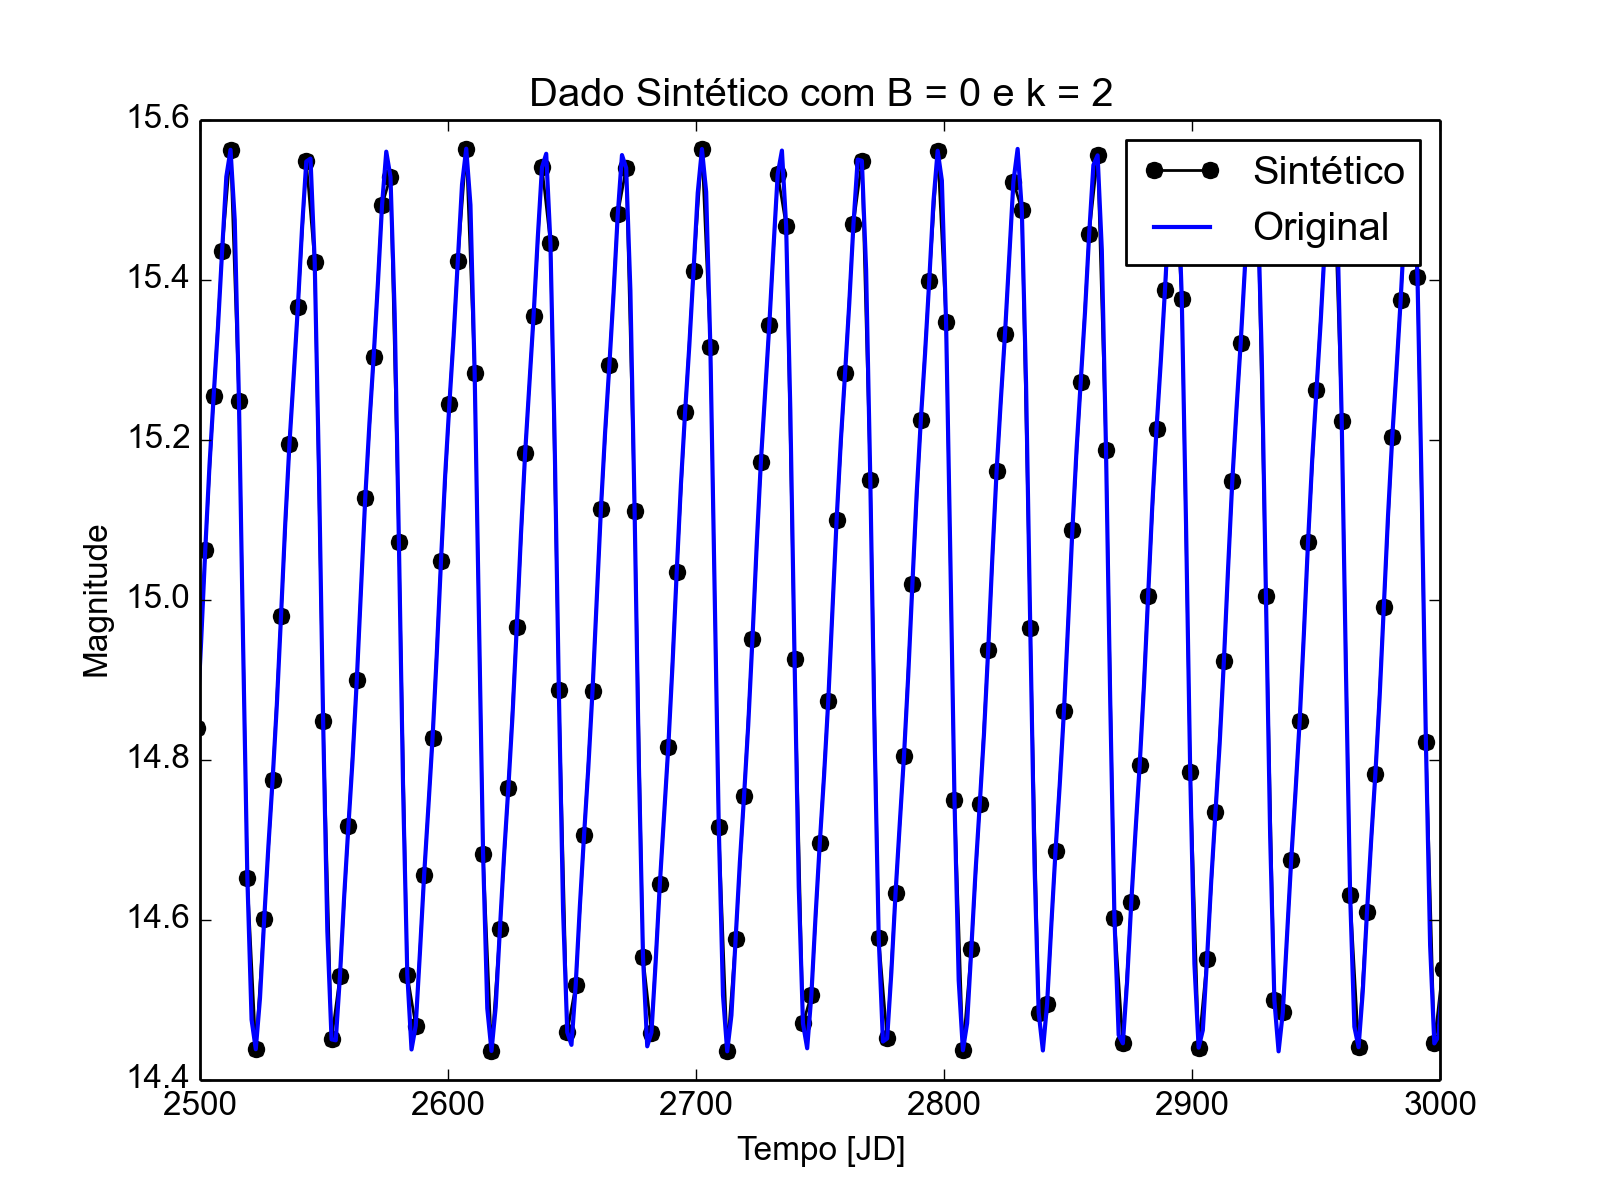
\includegraphics[width=\linewidth]{dado_sintetico_0_ruido_2_amos.png}
  \caption{Dado sem ruído e $k=2$}
  \label{fig:2amos}
  \end{subfigure}
\\
\begin{subfigure}{.5\textwidth}
  \centering
  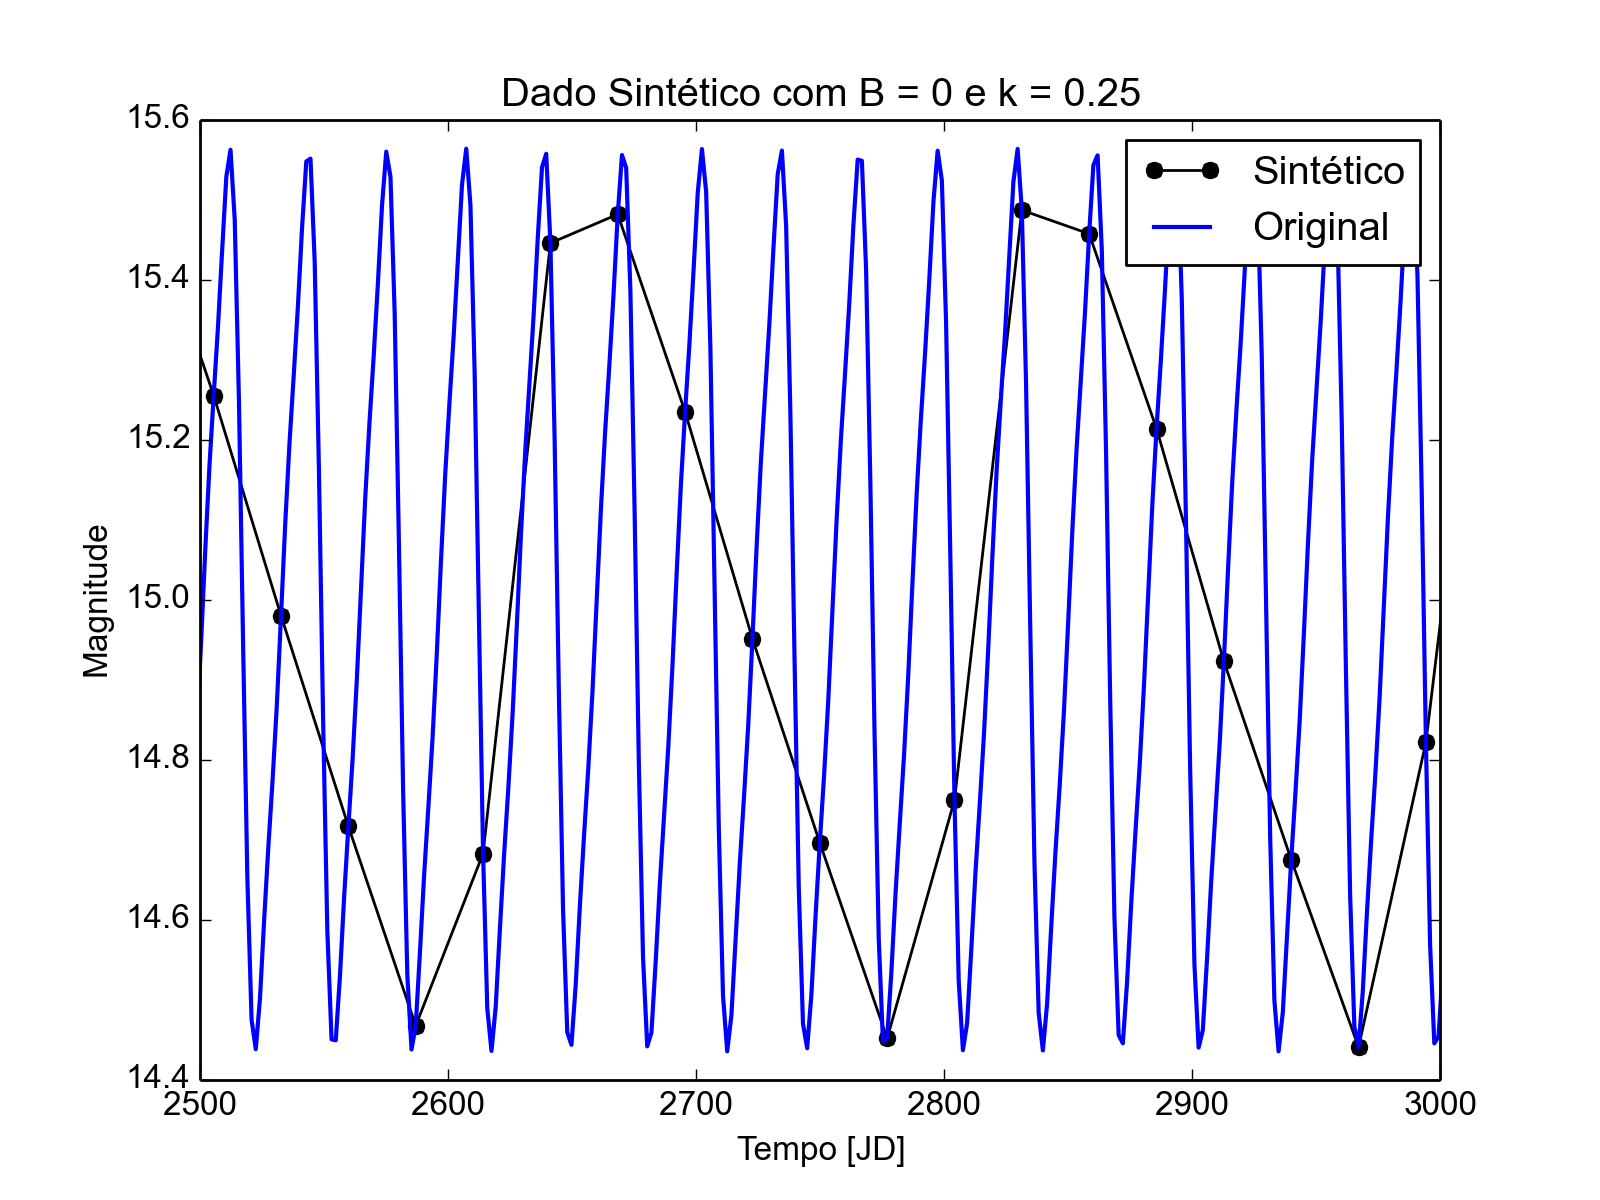
\includegraphics[width=\linewidth]{dado_sintetico_0_ruido_0_25_amos.png}
  \caption{Dado sem ruído e $k=1/4$}
  \label{fig:025amos}
\end{subfigure}%
\begin{subfigure}{.5\textwidth}
  \centering
  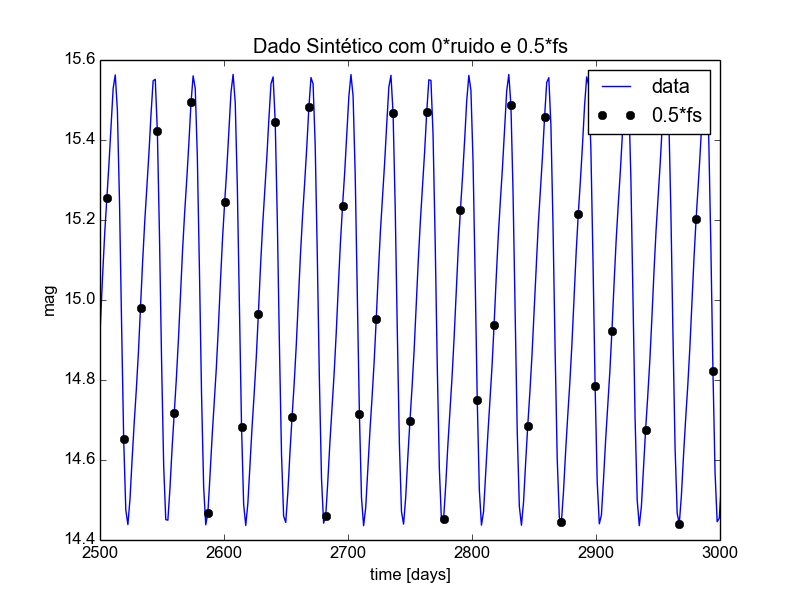
\includegraphics[width=\linewidth]{dado_sintetico_0_ruido_0_5_amos.png}
  \caption{Dado sem ruído e $k=1/2$}
  \label{fig:05amos}
  \end{subfigure}
\caption[Curva de luz sintética.]{Exemplos de curvas de luz sintética. Os exemplos foram criados sem ruído, $B=0$, e variando $k$. A linha azul representa o sinal original completo e os pontos e linha preta correspondem a observação com a amostragem $k$.}
\label{fig:exemplo_curva_luz}
\end{figure}


Para estudar a influência da amostragem nos dados, o vetor $t$ será criado utilizando os valores obtidos pelos histogramas de tempo inicial ($t_i = 2152,5019$) e final ($t_f = 4539,4593$) e a variação de pontos $dt$ será construído pela relação:
\begin{align}
dt = \frac{1}{f}
\end{align}
Em que $f = k \times f_s$, ou seja, a frequência de pontos $f$ será um parâmetro de escala $k$ vezes a amostragem $f_s$ dos dados. Desta forma, variando o parâmetro $k$ de $0,25$ a $4,0$ com um intervalo de $0,25$ e variando o parâmetro de escala para o ruído $B$ de $0,0$ até $1,0$ com intervalo de $0,05$, foram criadas 300 curvas de luz para serem analisadas. Quatro exemplos de curva de luz sintética gerada pelo método acima podem ser vistas na figura \ref{fig:exemplo_curva_luz}.




Na figura \ref{fig:exemplo_curva_luz}, os pontos e linha preta correspondem aos pontos de observação e a linha contínua azul seria o sinal original completo. Podemos perceber que quanto maior a amostragem, maior a quantidade de pontos.

\begin{figure}[H]
\centering
\hspace{-2.5cm}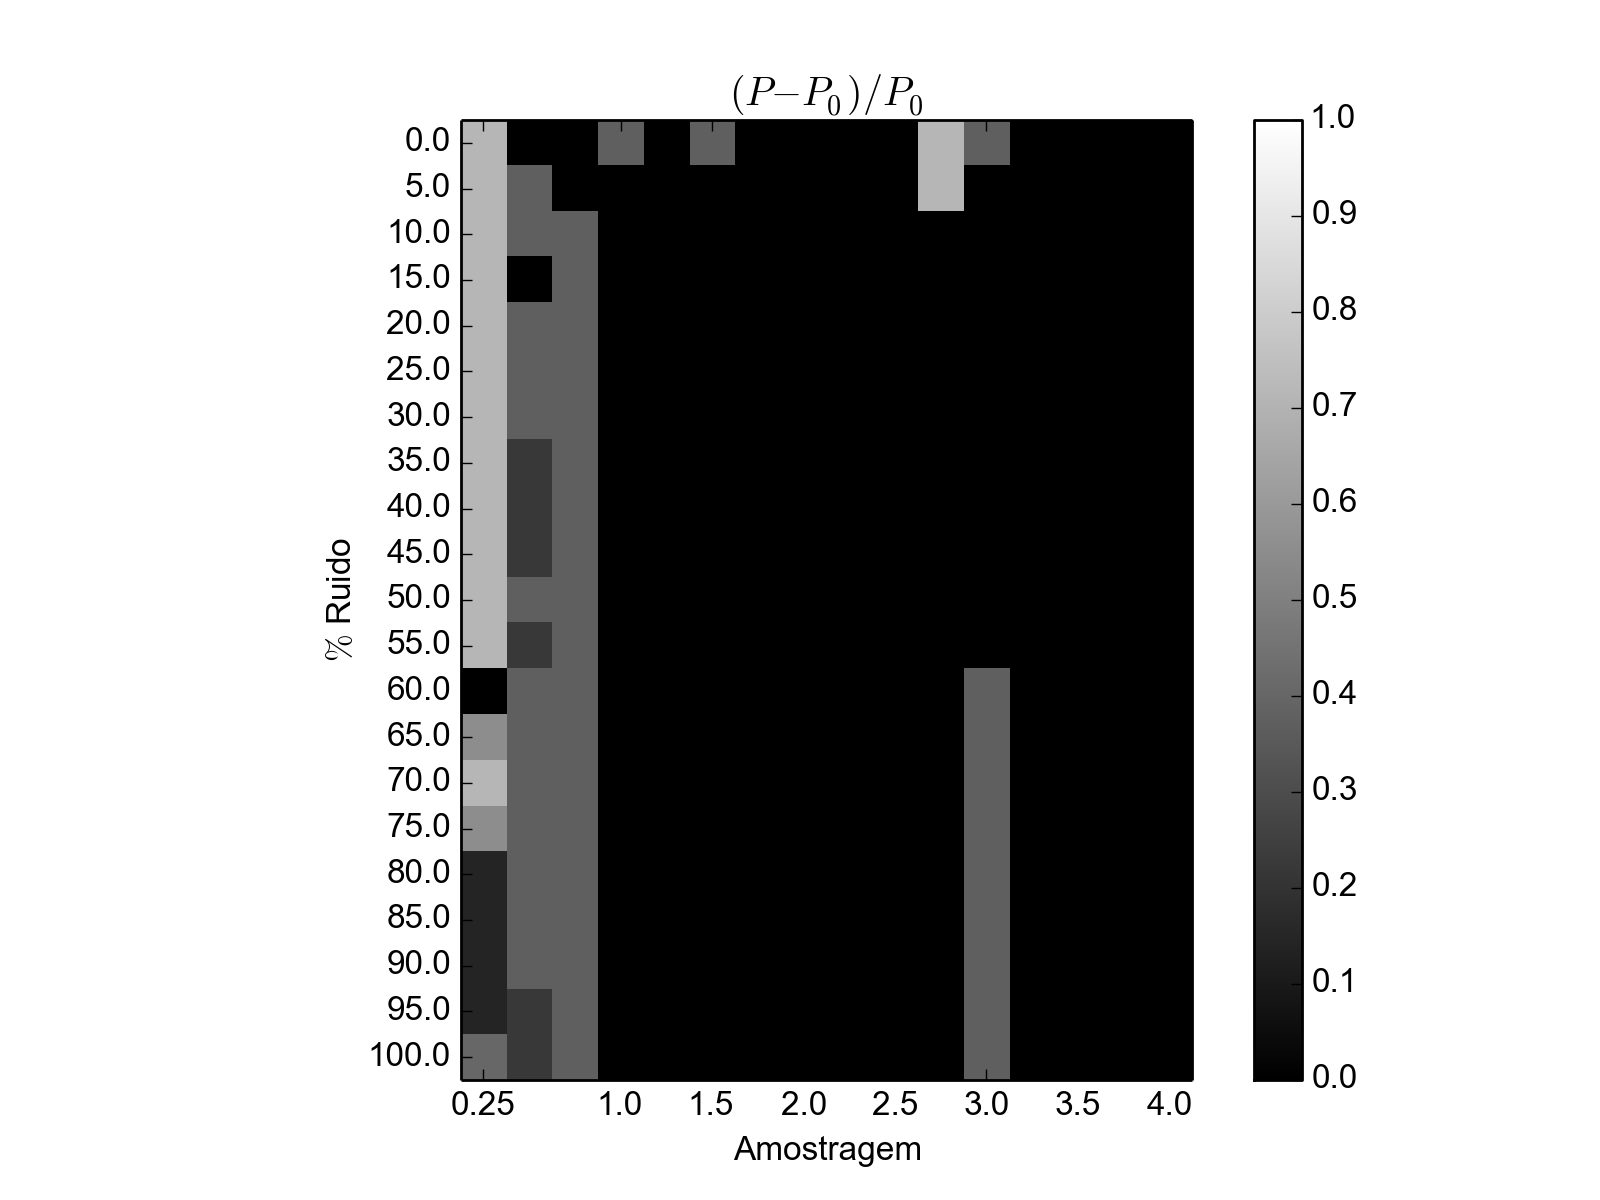
\includegraphics[scale=.8]{ce_inshow.png}
\caption[Resultados obtidos em escala de cinza.]{Resultados obtidos em escala de cinza. O eixo das abcissas representa o parâmetro de escala $k$ da amostragem e o eixo das ordenadas representa a variação do parâmetro de escala $B$ para o ruído. Quanto mais escura a cor do quadrado mais correto o valor calculado pela entropia de Shannon condicional.}
\label{fig:imshow}
\end{figure}

A figura \ref{fig:imshow} nos mostra um mapa de cor em escala de cinza entre parâmetro de escala $B$ do ruído e o parâmetro de escala $k$ da amostragem. A cor representa o valor $|(P - P_0)/P_0|$, ou seja, quanto o período calculado está variando em relação ao período original. A cor mais escura representa o valor 0 (período calculado = período real) e quanto mais clara a cor, maior o desvio do período.



%Obtendo a amostragem, podemos construir dados sintéticos variando a amostragem e o nível de ruído afim de estudar o comportamento do método. De acordo com \cite{ce} e \cite{entropy}, para construir dados sintéticos semelhantes com os dados observacionais da maioria dos Surveys de estrelas variáveis, podemos utilizar a seguinte expressão,
%\begin{align}
%m(t) &= A_0 + \sum_i^3 A_n \sin \Big( \frac{2 k \pi t}{P} \Big) + B \eta
%\end{align}
%em que $B$ é um fator de escala para o ruido entre \(0.0\) e \(1.0\), \(\eta\) é uma distribuição gaussiana com média zero e desvio unitário e \(P\) é o período médio das RRlyraes que, segundo \cite{lyraes} é de \(0.576\) dias.
%
%A influencia da amostragem está no vetor \(t\) que é construindo a fim de representar de forma mais fiel possível os dados do Catálogo OGLE-III. Sendo assim, o vetor tempo é construído com os seguinte parâmetros: tempo inicial de \(2152.5019\) HJD, tempo final de \(4539.4593\) HJD e espaçamento entre os pontos \(dt = 1 / f\) em que \(f = k \times f_s\) e \(k\) é um parâmetro de escala para a amostragem. Os tempos iniciais e finais foram escolhidos desta forma por serem os valores de maior frequência entre os dados das RRLyraes. Quatro exemplos de curva de luz sintética gerada pelo método acima podem ser vistas na figura \ref{fig:exemplo_curva_luz}.
%
%\begin{figure}[H]
%\centering
%\begin{subfigure}{.5\textwidth}
%  \centering
%  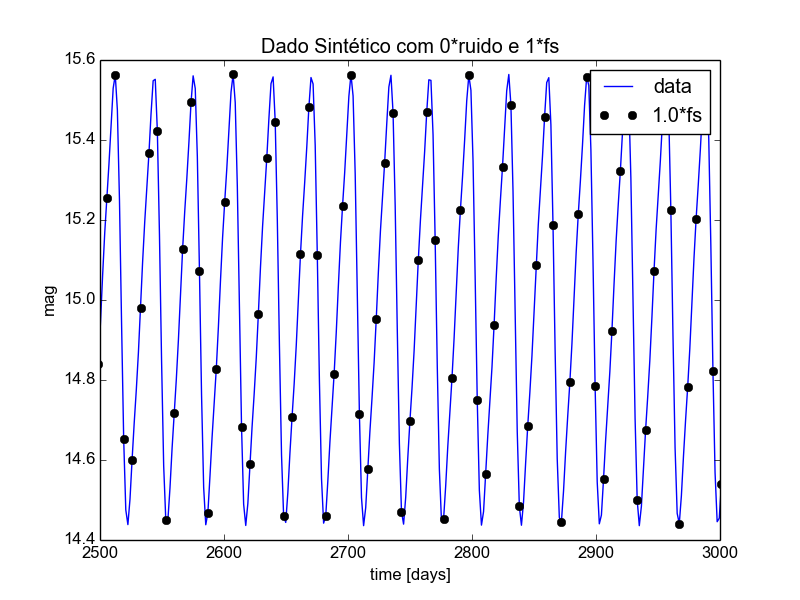
\includegraphics[width=\linewidth]{dado_sintetico_0_ruido_1_amos.png}
%  \caption{Dado sem ruído e com amostragem padrão}
%  \label{fig:1amos}
%\end{subfigure}%
%\begin{subfigure}{.5\textwidth}
%  \centering
%  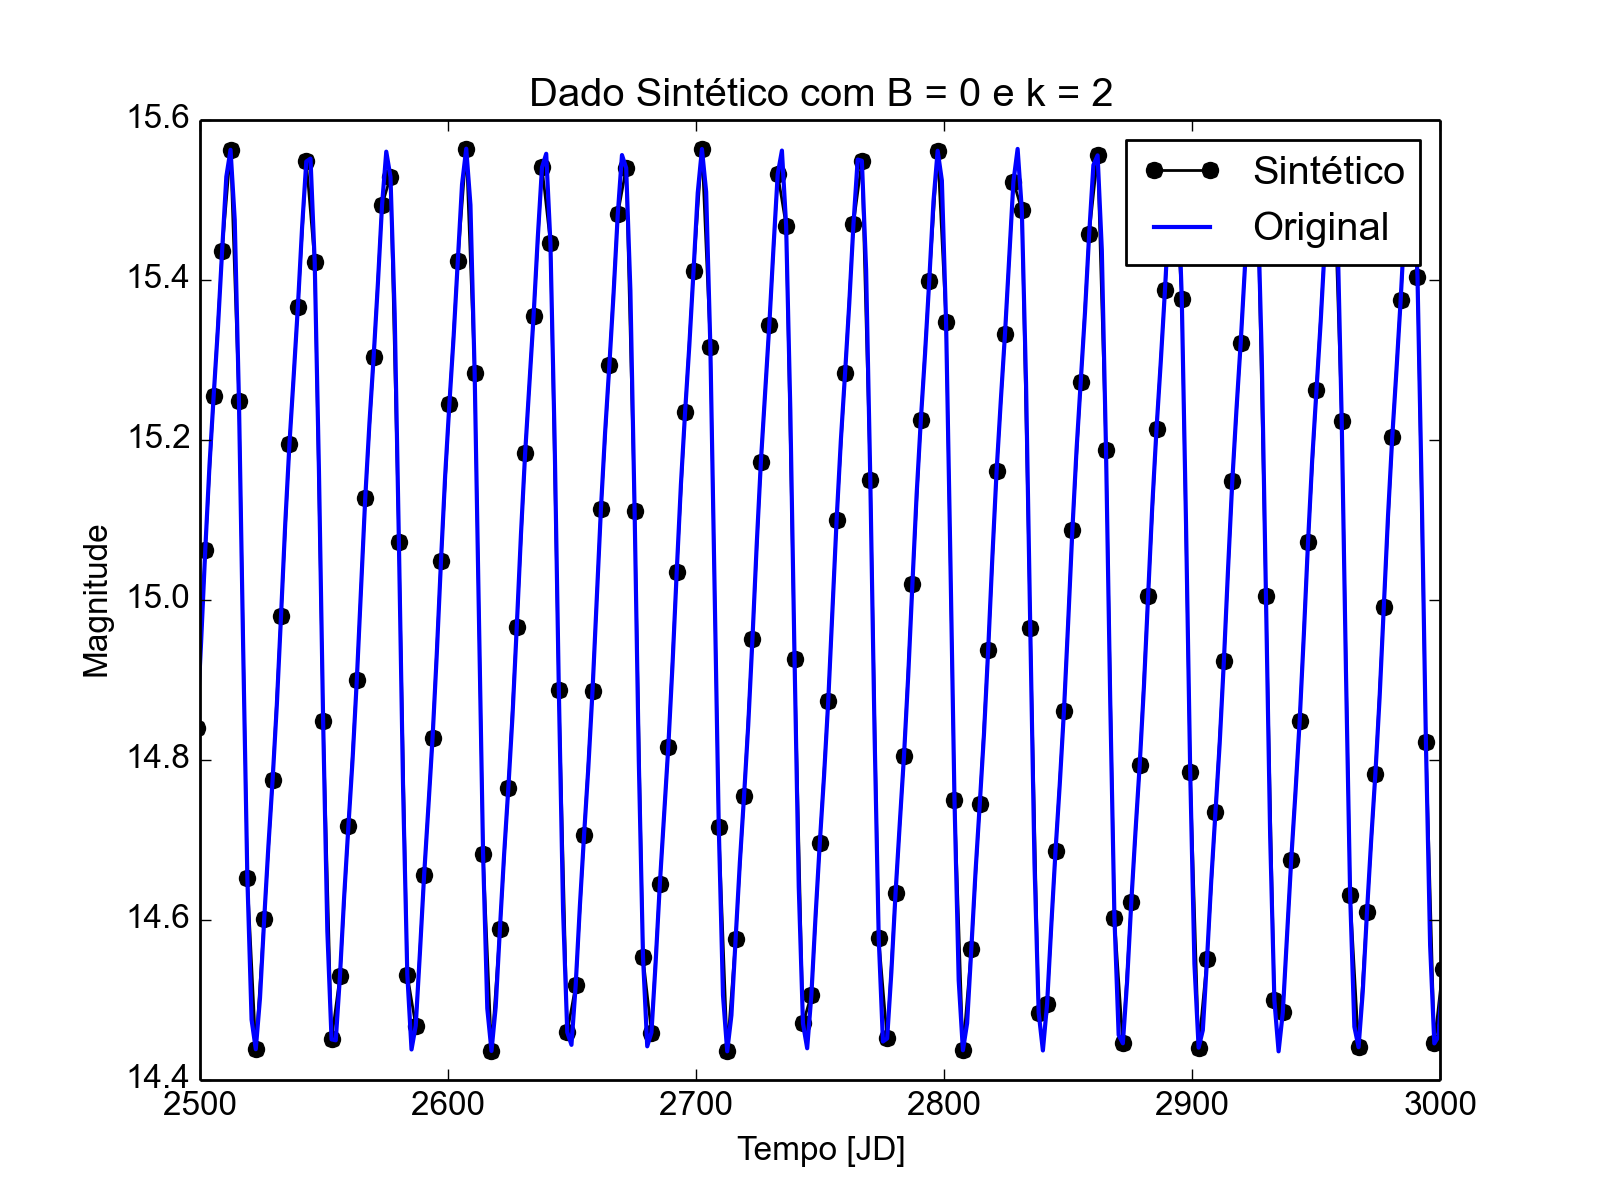
\includegraphics[width=\linewidth]{dado_sintetico_0_ruido_2_amos.png}
%  \caption{Dado sem ruído com $n=2$}
%  \label{fig:2amos}
%  \end{subfigure}
%\\
%\begin{subfigure}{.5\textwidth}
%  \centering
%  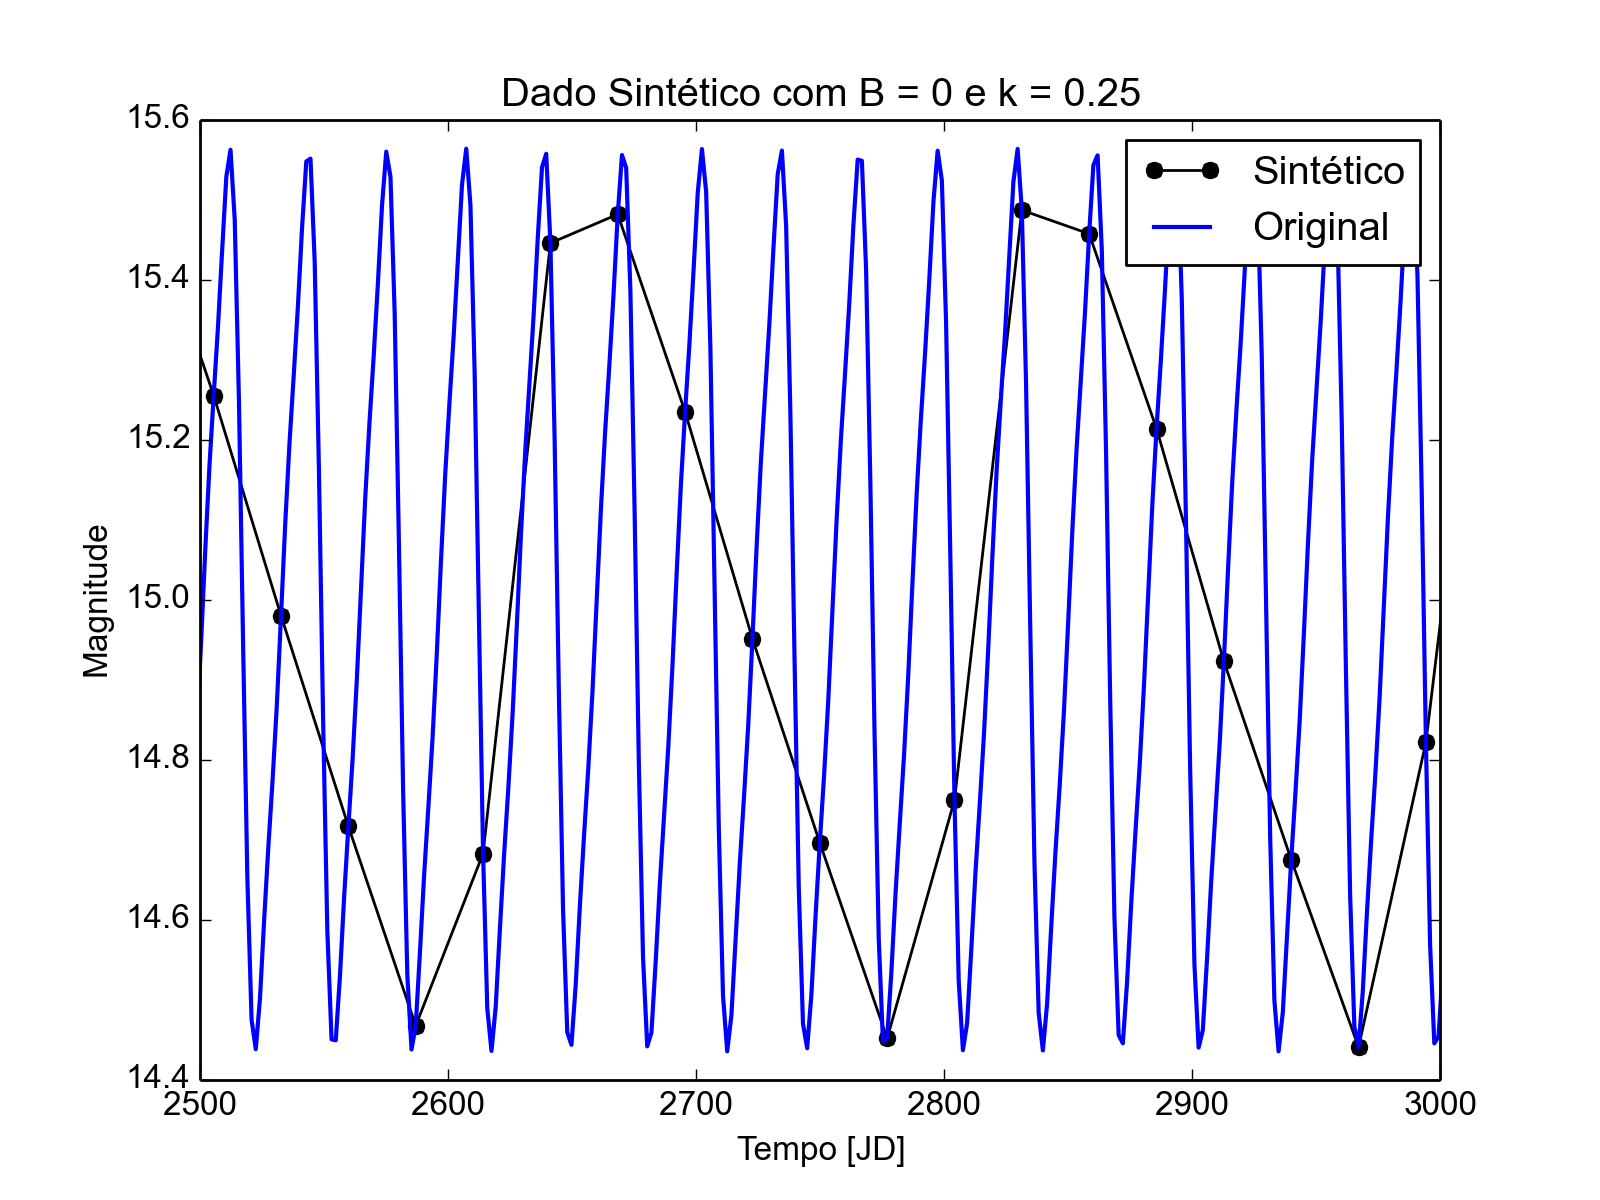
\includegraphics[width=\linewidth]{dado_sintetico_0_ruido_0_25_amos.png}
%  \caption{Dado sem ruído e com $n=1/4$}
%  \label{fig:025amos}
%\end{subfigure}%
%\begin{subfigure}{.5\textwidth}
%  \centering
%  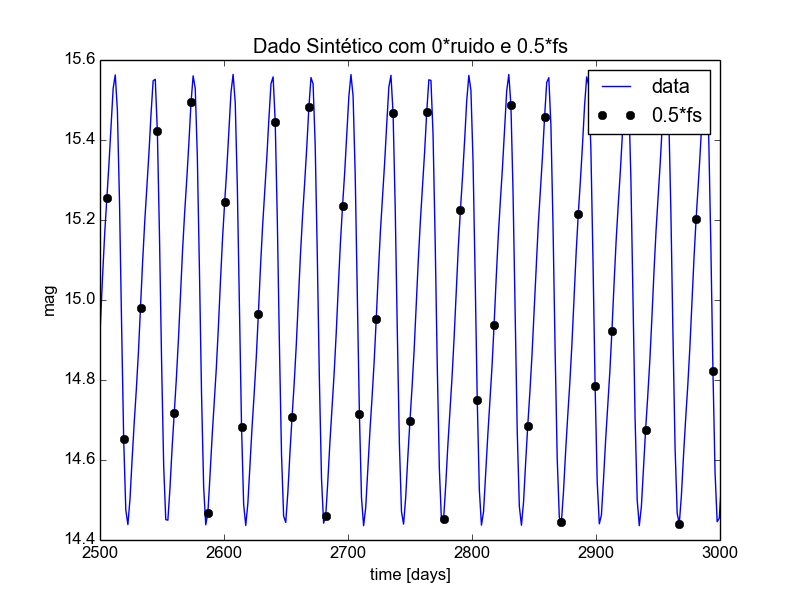
\includegraphics[width=\linewidth]{dado_sintetico_0_ruido_0_5_amos.png}
%  \caption{Dado sem ruído com $n=1/2$}
%  \label{fig:05amos}
%  \end{subfigure}
%\caption{Exemplos curva de luz sintética}
%\label{fig:exemplo_curva_luz}
%\end{figure}
%
%Na figura \ref{fig:exemplo_curva_luz}, os ponto pretos são os pontos de observação e a linha contínua é o dado original com \(n=1\). Podemos perceber que quanto maior a amostragem, maior a quantidade de pontos, assim o método aplicado a um dado com uma grande amostragem deve retornar um período com maior precisão do que comparado à um dado com pequena amostragem.

%Então, para estudar a influencia da amostragem nos dados foram gerados dados sintéticos variando o parâmetro $k$ da amostragem de $0.25$ a $4$ com intervalo de $0.25$ e variando o fator de escala $B$ de $0.0$ até $1.0$ com intervalo de $0.05$ assim obtendo $300$ curvas de luz. No momento, estamos pensando em como demonstrar os resultados obtidos. Uma forma para demonstrar os dados é fazendo um mapa de cor entre ruído e amostragem onde a cor representa o valor \(|(P - P_0)/P_0|\), ou seja, quanto que o período calculado está variando em relação ao período original. O mapa de cor é feito em escala de cinza, em que a cor mais escura representa o valor 0 (período calculado = período real) e quanto mais clara a cor, maior o desvio do período.	%o período calculado menos o período real do sinal dividido pelo período real, em  uma escala de cinza.



Podemos observar que a partir do parâmetro de escala $k=1,0$ para a amostragem, todos os resultado calculados foram corretos, não importando o nível de ruído, com exceção da faixa entre os ruídos $60\%$ e $100\%$ para $k=3$ que apresentam um resultado $\approx 0,4$. Essa exceção significa que o resultado obtido é aproximadamente a metade do período real.


%Os valores iguais a zero (cor preta) representam as configurações em que o método de entropia condicional calculou o período corretamente.

\section{Aplicação dos Resultados}

A grande importância da determinação de períodos de estrelas variáveis está na possibilidade de calcular distâncias a partir da Lei de Leavitt. Desta forma, utilizando a equação \ref{eq:leavitt_law} para magnitude médias, ou seja,
\begin{align}
\bar{M_i} = a \log P_i + b
\end{align}
e convertendo para a magnitude aparente média através da equação \ref{eq:dist_ext}, %para o módulo de distância,
\begin{align}
\bar{m_i} = a \log P_i + b + \mu_i + A_{\lambda_i} \label{eq:cap4_pl}
\end{align}
é possível calcular as constantes $a$ e $b$ utilizando o método dos mínimos quadrados para obter a relação entre o período e a luminosidade aparente. A correção para a extinção interestelar $A_\lambda$ é dada pelo mapa de \citet{Pejcha2009}.


Segundo \citet{Nikolaev2004}, o termo $\mu_i$ na equação \ref{eq:cap4_pl} pode ser escrito em duas partes:
\begin{align}
\mu_i = \bar{\mu} + \Delta \mu_i \label{eq:cap4_mod_dist}
\end{align}
Em que $\bar{\mu}$ é o modulo de distância médio para toda a Grande Nuvem de Magalhães e $\Delta \mu_i$ é a variação na distância para cada estrela. Portanto, podemos reescrever a equação \ref{eq:cap4_pl} como:
\begin{align}
\bar{m_i} = a \log P_i + b^\prime + \Delta \mu_i + A_{\lambda_i}
\end{align}
Em que o termo $\bar{\mu}$ foi incorporado na nova constante $b^\prime$.
Os resultados obtidos para essas constantes utilizando o método dos mínimos quadrados são apresentados na tabela \ref{tab:pl_relacao} para os 4 tipos de estrelas utilizados neste trabalho. As figuras \ref{fig:pl_cep} e \ref{fig:rr_pl} mostram a relação calculada sobre os dados.

\begin{table}[ht]
\begin{center}
\caption{Constantes da Relação PL.}
\begin{tabular}{c|c|c}
\toprule%\hline
Objeto & $a$ & $b^\prime$ \\
\midrule%\hline
Cefeida FU & $-1,292$ & $16,878$ \\
Cefeida FO & $-1,573$  & $16,558$ \\
RR Lyrae AB & $-0,721$ & $18,363$\\
RR Lyrae C & $-0,022$ & $18,841$\\
\bottomrule%\hline
\end{tabular} \\
\label{tab:pl_relacao}
\end{center}
\end{table}



Obtendo essas relações, é possível calcular a variação na distância $\Delta \mu_i$ de cada uma das estrelas pelo residual entre a Lei de Leavitt e a magnitude média obtida pelos dados do catálogo, ou seja,
\begin{align}
\Delta \mu_i = \bar{m}_{OGLE} - \bar{m_i}
\end{align}
e o modulo de distância real é obtida pela equação \ref{eq:cap4_mod_dist} considerando uma distância média de $50\si{kpc}$ ou $\bar{\mu} = 18,495$ \citep{Pejcha2009}. Tendo calculado o modulo de distância para todas as estrelas, a distância é obtida pela equação \ref{eq:dist_vela_padrao} em Parsec.


\begin{figure}[ht]
\centering
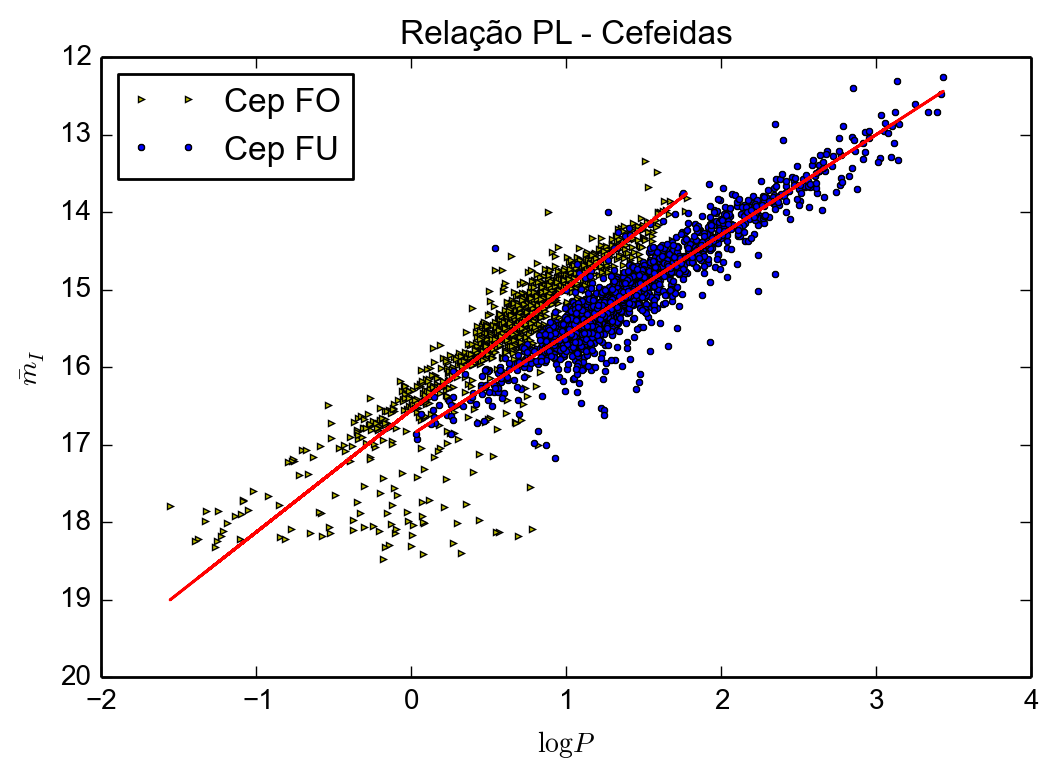
\includegraphics[width=0.6\linewidth]{cep_relacaoPL.png}
\caption[Relação PL para Cefeidas.]{Relação PL para as Cefeidas tipo FU e FO. O eixo das abcissas representa o logaritmo dos períodos calculados utilizando o método de entropia de Shannon condicional. O eixo das ordenadas representas a magnitude média de cada estrela na banda I obtidos no catálogo OGLE.}
\label{fig:pl_cep}
\end{figure}
%utilizando a equação \ref{eq:dist_ext} da seguinte forma: Sendo o modulo da distância dado pela relação,
%\begin{align}
%\mu = m - M - A_\lambda
%\end{align}
%e a magnitude absoluta obtida pela lei de Leavitt,
%\begin{align}
%M = a \log P + b
%\end{align}
%substituindo $M$ no modulo da distância,
%\begin{align}
%\mu = m - a \log P - b - A_\lambda
%\end{align}
\begin{figure}[!ht]
\centering
\begin{subfigure}{.5\textwidth}
  \centering
  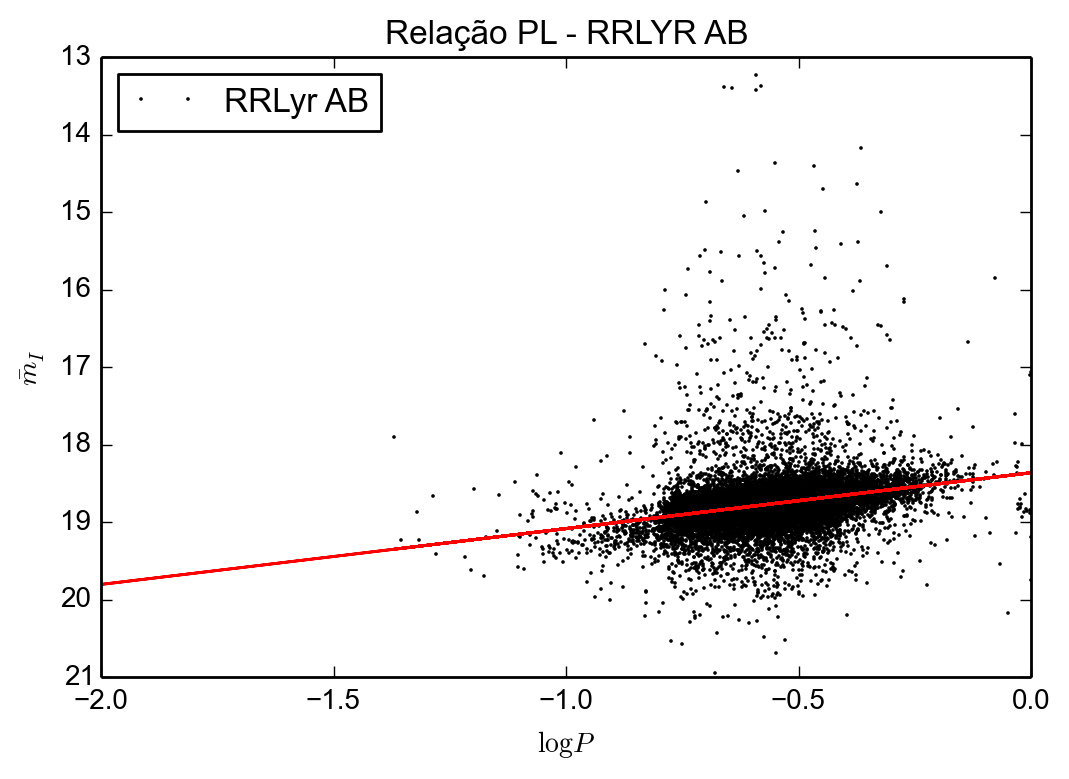
\includegraphics[width=\linewidth]{rrab_relacaoPL.png}
  \caption{RR Lyraes AB}
  \label{fig:ab_pl}
\end{subfigure}%
\begin{subfigure}{.5\textwidth}
  \centering
  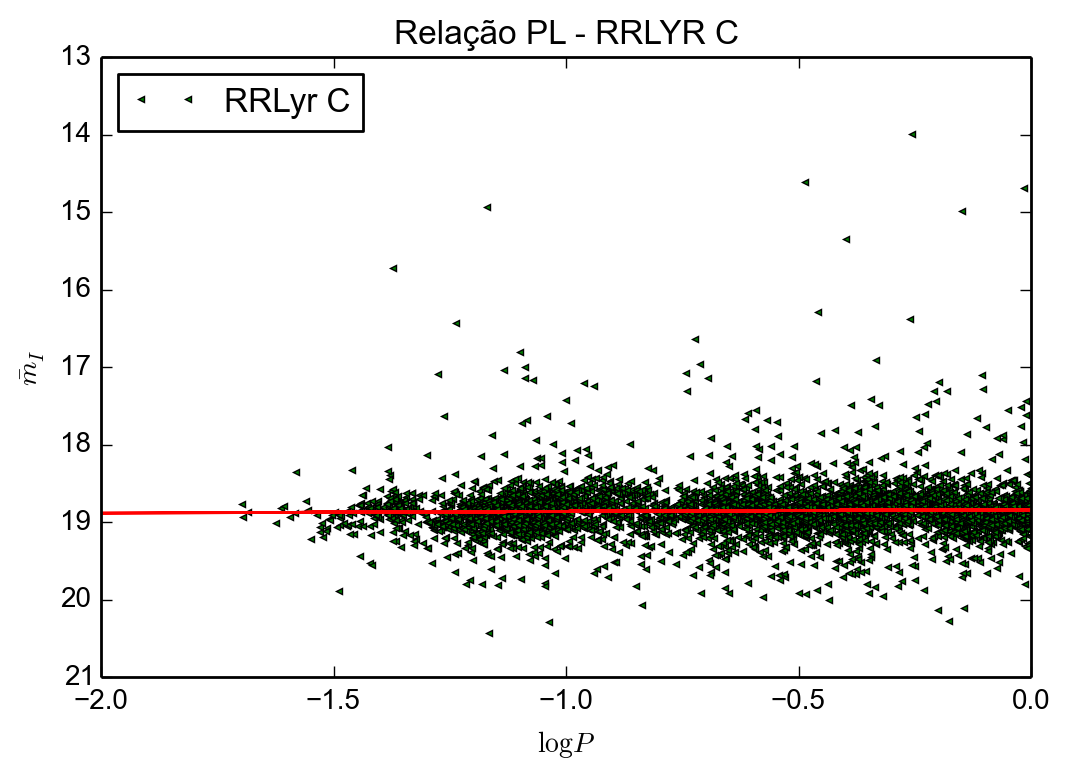
\includegraphics[width=\linewidth]{rrc_relacaoPL.png}
  \caption{RR Lyraes C}
  \label{fig:c_pl}
  \end{subfigure}
\caption[Relação PL para RR Lyraes.]{Relação PL para as estrelas RR Lyraes tipo AB (esquerda) e C (direita). O eixo das abcissas representa o logaritmo dos períodos calculados utilizando o método de entropia de Shannon condicional. O eixo das ordenadas representas a magnitude média de cada estrela na banda I obtidos no catálogo OGLE.}
\label{fig:rr_pl}
\end{figure}
%e isolando a magnitude
%\begin{align}
%m  = a \log P + b + A_\lambda + \mu
%\end{align}
%\textcolor{red}{continuar...}

Para determinar a estrutura da Grande Nuvem de Magalhães é necessário calcular a distribuição em coordenadas cartesianas a partir dos dados de ascensão reta ($\alpha$) e declinação ($\delta$) obtidos do catálogo OGLE e dos dados de distância ($r$) calculados anteriormente. Desta forma, será feita a transformação de um espaço de coordenadas ($\alpha$, $\delta$, $r$) para as coordenadas ($x$, $y$, $z$) considerando que a Grande Nuvem de Magalhães é centrada nas posições ($\alpha_0$, $\delta_0$, $r_0$). As transformações de coordenadas são dadas por \citet{Deb2014} e mostradas a seguir:
\begin{align}
x &= -r \sin \left(\alpha - \alpha_0 \right) \cos \left( \delta \right) \notag \\
y &= r \sin \left( \delta \right) \cos \left( \delta_0 \right) - r \sin \left( \delta_0 \right) \cos \left( \alpha - \alpha_0 \right) \cos \left( \delta \right) \label{eq:cap4_trans}\\
z &= r_0 - r \sin \left( \delta \right) \sin \left(\delta_0 \right) - r \cos \left( \delta_0 \right) \cos \left( \alpha \right) - \alpha_0 \cos \left( \delta \right) \notag
\end{align}

%\begin{align}
%x = -D \sin (\alpha - \alpha_0) \cos(\delta) \\
%y = D \sin (\delta) \cos (\delta_0) − D \sin (\delta_0) \cos (\alpha - \alpha_0) \cos( \delta) \\
%z = D_0 - D \sin(\delta)\sin(\delta_0) - D \cos (\delta_0) \cos( \alpha ) - \alpha_0 \cos (\delta)
%\end{align}

O centro da Grande Nuvem de Magalhães é obtido a partir dos valores médios das coordenadas equatoriais $\alpha$ e $\delta$ e possui valores $\alpha_0 = 80,240^\circ$ e $\delta_0 = -69.608^\circ$, como mostrado na figura \ref{fig:equatorial}.

\begin{figure}[!ht]
\centering
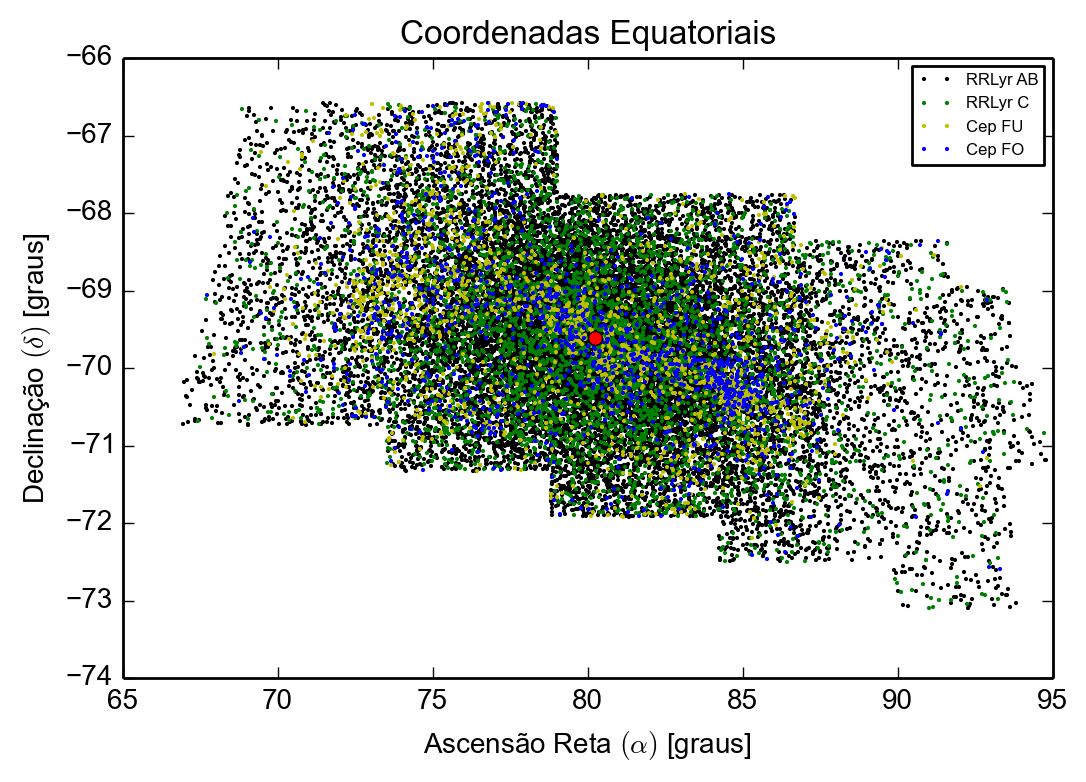
\includegraphics[width=0.6\linewidth]{equatorial.png}
\caption[Distruibuição de estrelas em coordenadas equatoriais.]{Distribuição das posições das estrelas do pulsantes do catálogo OGLE em coordenadas equatoriais. O ponto vermelho no centro representa a centroide e possui posição $\alpha_0 = 80,240^\circ$ e $\delta_0 = -69,608^\circ$.}
\label{fig:equatorial}
\end{figure}

Assim, utilizando as transformações \ref{eq:cap4_trans} foi calculado a distribuição tridimensional da Grande Nuvem de Magalhães como mostra a figura \ref{fig:plot3d}.

\begin{figure}[!ht]
\centering
\begin{subfigure}{.5\textwidth}
\centering
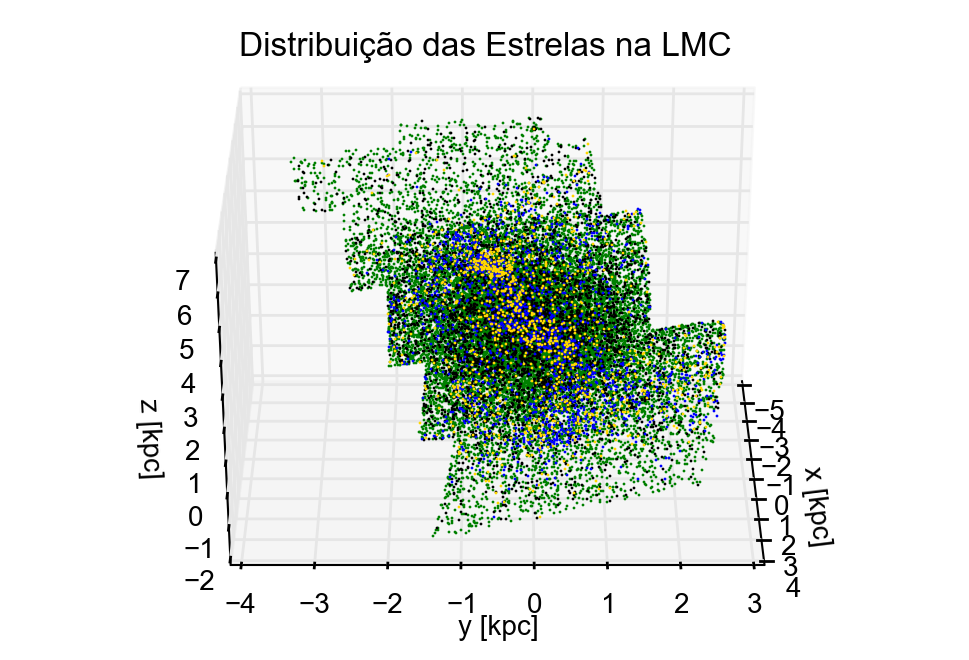
\includegraphics[width=\linewidth]{3d_plot_0.png}
\caption{0}
\end{subfigure}%
\begin{subfigure}{.5\textwidth}
\centering
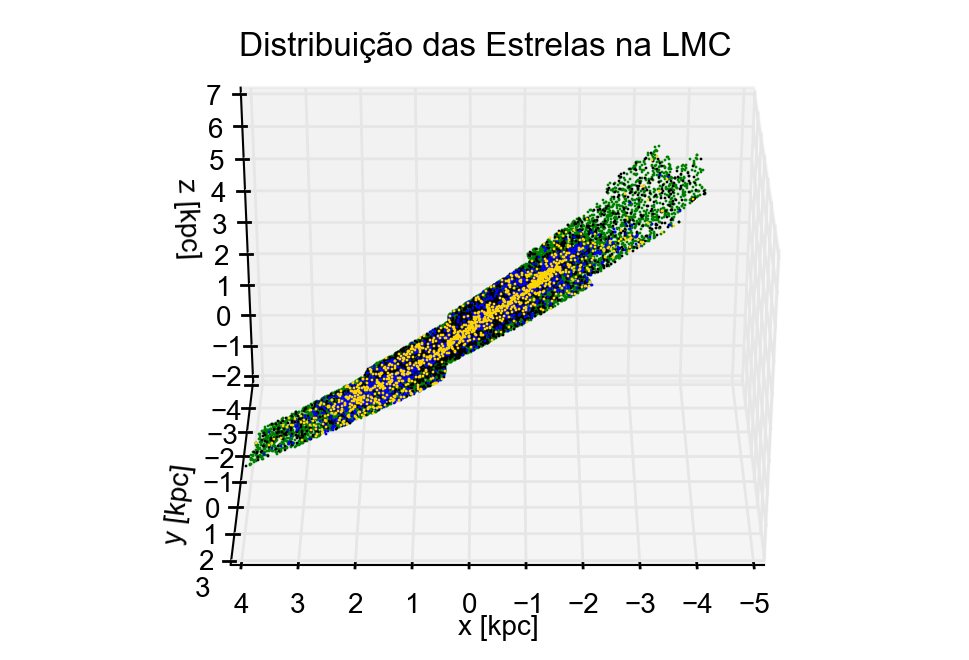
\includegraphics[width=\linewidth]{3d_plot_90.png}
\caption{90}
\end{subfigure}
\\
\begin{subfigure}{.5\textwidth}
\centering
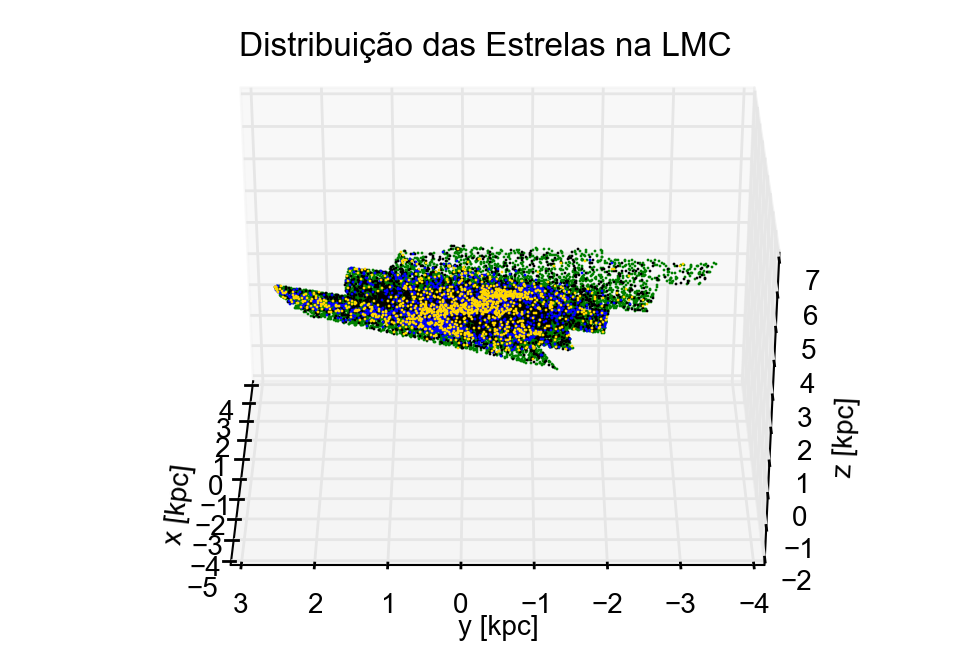
\includegraphics[width=\linewidth]{3d_plot_180.png}
\caption{180}
\end{subfigure}%
\begin{subfigure}{.5\textwidth}
\centering
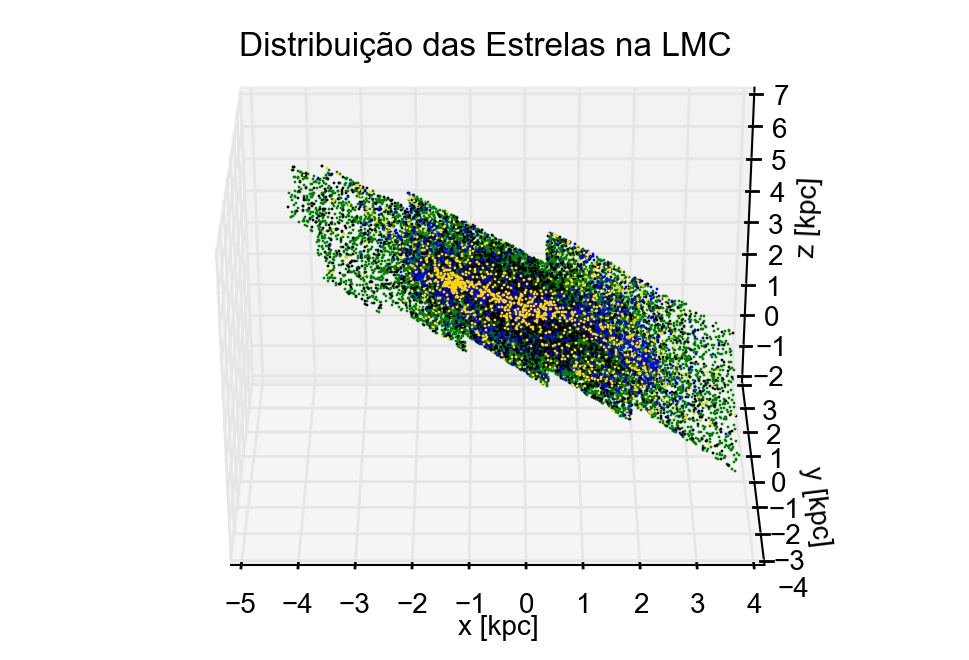
\includegraphics[width=\linewidth]{3d_plot_270.png}
\caption{270}
\end{subfigure}
%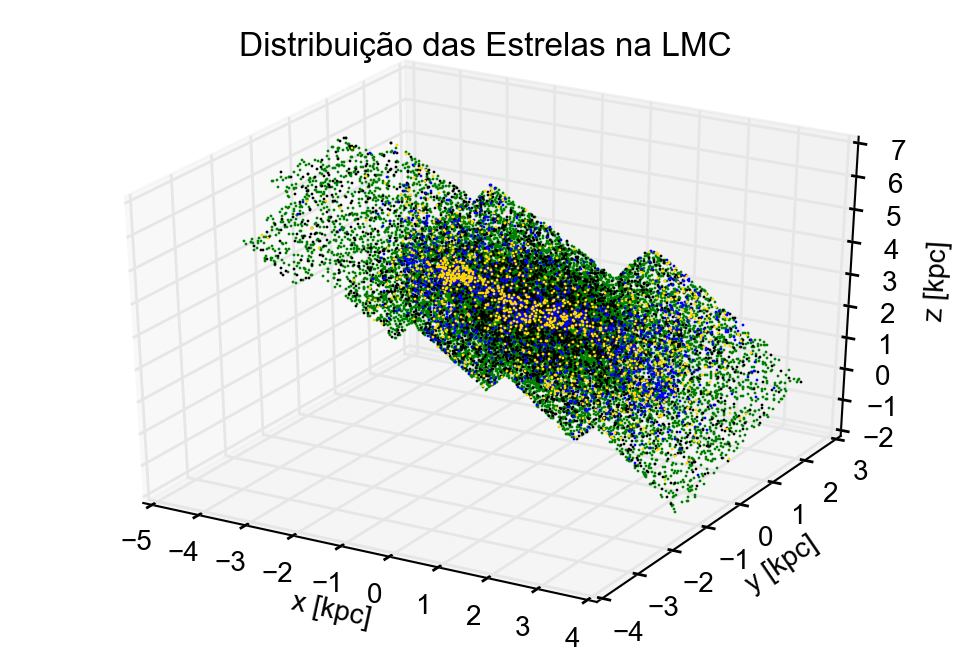
\includegraphics[width=0.8\linewidth]{plot3d.png}
\caption[Distruição 3D da Grande Nuvem de Magalhães.]{Distruição tridimensional da Grande Nuvem de Magalhães em coordenadas cartesianas. São mostradas a distruição em 4 ângulos de visão, $0^\circ$ (A), $90^\circ$ (B), $1800^\circ$ (C), $270^\circ$ (D) }
\label{fig:plot3d}
\end{figure}

Assim é possível perceber como a galaxia se distribui espacialmente e perceber que a maioria das estrelas se concentram na região central.

%\section{Conclusão}

%A observação e detecção de períodos de estrelas variáveis é fundamental para descrição desses objetos astronômicos e para a determinação de distâncias. Embora existam diversos métodos para o calculo de período, o desenvolvimento de técnicas que sejam confiáveis e possam ser aplicadas para dados com espaçamento variável entre os pontos de observação é de grande importância em uma realidade em que há dificuldades para observação dos telescópios, sendo essas dificuldades devido ao tempo disponível de observação e as condições climáticas. O método apresentado neste trabalho, a entropia de Shannon condicional, é uma técnica simples de ser entendida e aplicada, possuindo  um embasamento matemático dentro da teoria da informação, o que faz com que a sua análise estatística seja conhecida, fato que não é verdade para alguns métodos de detecção de períodos. Além disso, o método  apresenta um desempenho mais do que satisfatório com uma taxa de acerto maior do que $97\%$ para as $25707$ estrelas pulsantes do catálogo OGLE-III. Além disso, a análise dos dados sintéticos afirma que o método é confiável para qualquer nível de ruído desde que a frequência de pontos dos dados seja maior do que $f_s = 0,1473$. Por fim, com a figura \ref{fig:imshow} foi possível  construir uma ferramenta que nos indica como os dados influenciam no resultado do método, ou ainda, partindo do resultado que se espera obter, é possível determinar como a observação nos telescópios devem ser conduzidas. Parte dos resultados obtidos nesse trabalho foram apresentados em \citet{gabe1} e \citet{gabe2}.
